\documentclass[9pt]{article}
\usepackage{graphicx}
\usepackage{hyperref}
\usepackage{amsmath}
\usepackage{enumitem}
\usepackage{cite}
\usepackage[labelfont=bf]{caption}
\usepackage{float}
\usepackage{listings}
\usepackage{lstautogobble}

\lstset{basicstyle=\ttfamily,
  mathescape=true,
  escapeinside=||,
  autogobble}

% Copyright 2017 Sergei Tikhomirov, MIT License
% https://github.com/s-tikhomirov/solidity-latex-highlighting/

\usepackage{listings, xcolor}

\definecolor{verylightgray}{rgb}{.97,.97,.97}

\lstdefinelanguage{Solidity}{
	keywords=[1]{anonymous, assembly, assert, balance, break, call, callcode, case, catch, class, constant, continue, contract, debugger, default, delegatecall, delete, do, else, emit, event, export, external, false, finally, for, function, gas, if, implements, import, in, indexed, instanceof, interface, internal, is, length, library, log0, log1, log2, log3, log4, memory, modifier, new, payable, pragma, private, protected, public, pure, push, require, return, returns, revert, selfdestruct, send, storage, struct, suicide, super, switch, then, this, throw, transfer, true, try, typeof, using, value, view, while, with, addmod, ecrecover, keccak256, mulmod, ripemd160, sha256, sha3}, % generic keywords including crypto operations
	keywordstyle=[1]\color{blue}\bfseries,
	keywords=[2]{address, bool, byte, bytes, bytes1, bytes2, bytes3, bytes4, bytes5, bytes6, bytes7, bytes8, bytes9, bytes10, bytes11, bytes12, bytes13, bytes14, bytes15, bytes16, bytes17, bytes18, bytes19, bytes20, bytes21, bytes22, bytes23, bytes24, bytes25, bytes26, bytes27, bytes28, bytes29, bytes30, bytes31, bytes32, enum, int, int8, int16, int24, int32, int40, int48, int56, int64, int72, int80, int88, int96, int104, int112, int120, int128, int136, int144, int152, int160, int168, int176, int184, int192, int200, int208, int216, int224, int232, int240, int248, int256, mapping, string, uint, uint8, uint16, uint24, uint32, uint40, uint48, uint56, uint64, uint72, uint80, uint88, uint96, uint104, uint112, uint120, uint128, uint136, uint144, uint152, uint160, uint168, uint176, uint184, uint192, uint200, uint208, uint216, uint224, uint232, uint240, uint248, uint256, var, void, ether, finney, szabo, wei, days, hours, minutes, seconds, weeks, years},	% types; money and time units
	keywordstyle=[2]\color{teal}\bfseries,
	keywords=[3]{block, blockhash, coinbase, difficulty, gaslimit, number, timestamp, msg, data, gas, sender, sig, value, now, tx, gasprice, origin},	% environment variables
	keywordstyle=[3]\color{violet}\bfseries,
	identifierstyle=\color{black},
	sensitive=false,
	comment=[l]{//},
	morecomment=[s]{/*}{*/},
	commentstyle=\color{gray}\ttfamily,
	stringstyle=\color{red}\ttfamily,
	morestring=[b]',
	morestring=[b]"
}

\lstset{
	language=Solidity,
	backgroundcolor=\color{verylightgray},
	extendedchars=true,
	basicstyle=\footnotesize\ttfamily,
	showstringspaces=false,
	showspaces=false,
	%numbers=left,
	%numberstyle=\footnotesize,
	%numbersep=9pt,
	tabsize=2,
	breaklines=true,
	showtabs=false,
	captionpos=b
}

% wide margins
\addtolength{\oddsidemargin}{-.75in}
\addtolength{\evensidemargin}{-.75in}
\addtolength{\textwidth}{1.5in}
\addtolength{\topmargin}{-.875in}
\addtolength{\textheight}{1.75in}

\captionsetup[table]{skip=4pt}

\begin{document}

% START TITLE PAGE
\title{ \textbf{Paradigm: A Decentralized Relay Protocol for Smart Contract Based Financial Primitives} } 
\author{Liam Kovatch, Henry Harder \\ \\ \texttt{\{liam,henry@paradigm.market\}}} 
\date{\today}
\maketitle 
% END TITLE PAGE


%BEGIN ABSTRACT
\begin{abstract}

\noindent We motivate an infrastructure-level relay protocol and generalized forwarding contract interface system. Built on the Ethereum blockchain and an independent network of nodes, the system functions to support and incentivize an ecosystem of decentralized financial instrumentation and global liquidity. The protocol aims to reduce redundancies and fragmentation present in the current relayer model by replacing relayers with a generalized relay protocol. The model we propose creates a globally accessible event-stream based order book on which a network of order matchers and dApps can be built. The complete protocol creates a universal relay platform that abstracts liquidity from centralized venues to a public decentralized network. The architecture of this system provides a modular interface for contract logic that allows for the creation of diverse and synthetic markets. Paradigm aims to enable more efficient and inclusive global markets by building and incentivizing a public, trustless, and global liquidity pool hosted by market participants. The protocol will be free to use and open source, reducing barriers to entry for both developers and market agents. \\

\end{abstract}
\pagebreak
% END ABSTRACT


% TABLE OF CONTENTS
\tableofcontents
\pagebreak
% END TABLE OF CONTENTS


% BEGIN INTRO
\section{Introduction}\label{intro}

\noindent The digital tokenization of assets and use of blockchain technology for financial settlement offers significant advantages in trading and market efficiency over existing alternatives such as centralized clearinghouses and exchanges\cite{defi}. Projects such as 0x\cite{0xwhitepaper}, dY/dX\cite{dydxwhitepaper}, and Dharma\cite{dharmawhitepaper} have begun to capitalize on such efficiencies through the implementation of public/private key-pair cryptography, smart-contact based settlement logic, and the Ethereum platform. \\

\noindent The 0x Project defined a system in which a pipeline of publicly accessible Ethereum smart contracts facilitate the wallet-to-wallet exchange of funds\cite{0xwhitepaper}. In this model, the processes of order broadcast and discovery are the responsibility of third party, off-chain entities called relayers. Relayers are responsible for sourcing and maintaining liquidity in the form of independent collections of signed order messages. This architecture removes the friction and security risk of centralized custodial parties while maintaining the performance and structure necessary to support liquid and interoperable markets. \\

\noindent While the current relayer model solves the core problem of vulnerable centralized custodianship, trading still requires the involvement of centralized parties in order to facilitate order broadcast and discovery. The centralized management of order-booking systems also results in proprietary and fragmented liquidity\cite{globalliquidity, eufinance}. In addition to creating general market inefficiencies, this model makes exchange difficult for traders that are in crypto antagonistic locales or are looking to trade non-traditional instruments and assets\cite{relayerideas}. More generally, the current market structure results in redundant systems between relayers, and the creation of unnecessary barriers between potential traders and developers. \\

\noindent We propose an abstraction of this system via the creation of a new middleware protocol and accompanying network infrastructure. Paradigm’s solution iterates on the current relayer model by introducing a decentralized relay network and protocol to facilitate low friction order broadcast and discovery. The protocol transfers the roles of order relay and liquidity management from centralized venues to a performant decentralized network. \\

\clearpage
\pagebreak
% END INTRO 

% BEGIN SCHEMATIC SECTION
\section{Protocol Schematic and Overview}\label{schematic}

\noindent In its most general sense, the Paradigm Protocol serves as a middleware component for hybrid decentralized settlement logic built on Ethereum. Situated between smart contract based settlement logic and end-user systems, the protocol and underlying network function to distribute liquidity, simplify the decentralized exchange stack, motivate the creation of diverse smart contract exchange logic, and enable the creation of an unrestricted global liquidity pool. Figure \ref{fig:fig1} presents a simplified visualization of the decentralized exchange stack as motivated by the Paradigm Protocol. 

\begin{figure}[H]
    \centering
    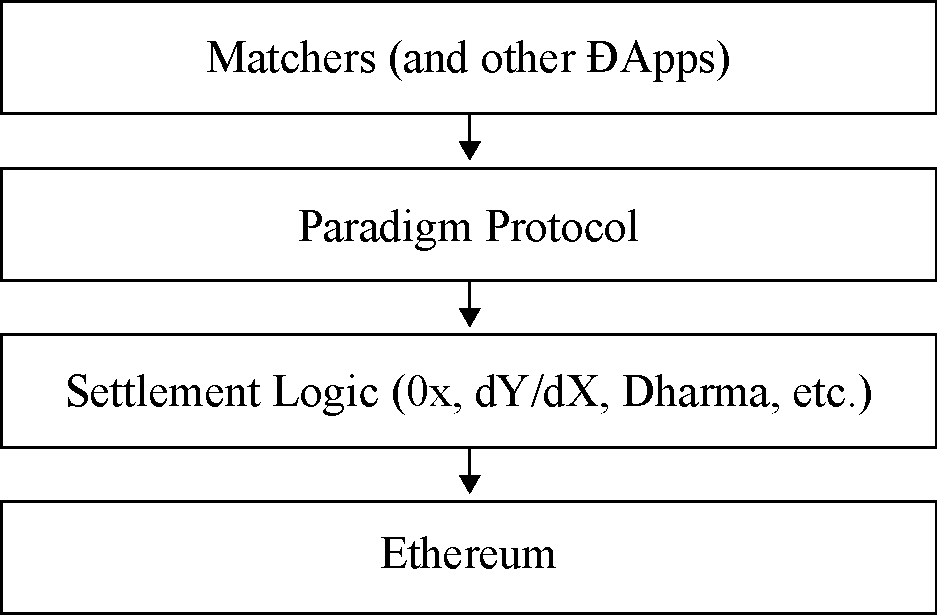
\includegraphics[scale=0.35]{../figures/fig1.pdf}
    \caption{A simplified application stack diagram of the Paradigm decentralized exchange model.}
    \label{fig:fig1}
\end{figure}

\noindent The operational flow of the Paradigm Protocol can be broken into a generalized sequence of steps\footnote{Many of these steps can and likely will be abstracted from end users by applications building on the Paradigm Protocol.}. Figure \ref{fig:fig2} presents a visual representation of these steps, and is followed by a brief description of this sequential process. 

\begin{figure}[H]
    \centering
    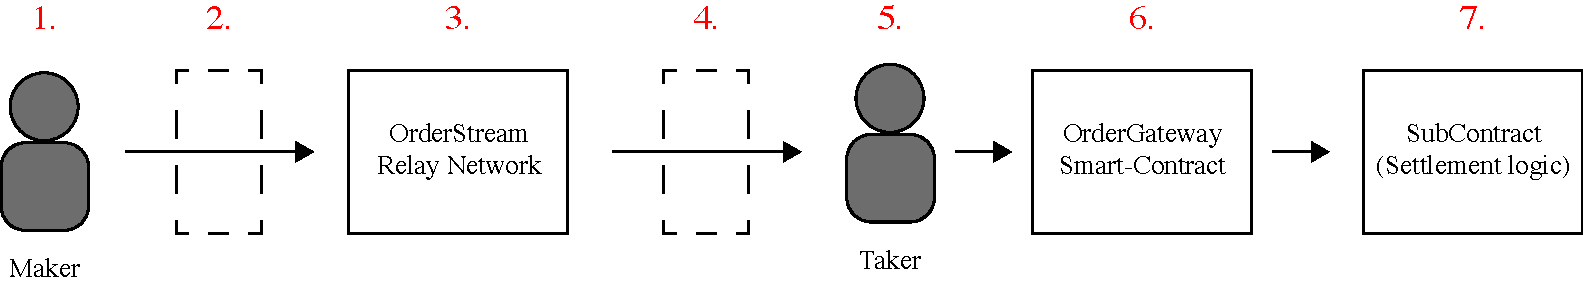
\includegraphics[scale=0.5]{../figures/fig2.pdf}
    \caption{Generalized exchange flow showing maker/taker order placement and forwarding process (simplified). }
    \label{fig:fig2}
\end{figure}

\begin {enumerate}
\item A maker signs an order message, which includes the address of the targeted settlement smart-contract (SubContract), and the order data specific to that SubContract.
\item A poster signs the maker order (the poster may be the same as the maker) and submits the signed order to the relay network via the API provided by an OrderStream validator node.
\item The OrderSteam confirms the validity of the order, and if deemed valid by the network, each validator node broadcasts the order as an event via the WebSocket protocol.
\item A taker subscribed to the OrderStream discovers an order they wish to fill.
\item To fill this order, the taker submits a complete and signed order message to the OrderGateway contract.
\item The OrderGateway contract forwards the order data to the specified SubContract.
\item The order is settled via the specified SubContract.
\end{enumerate}

\noindent The following sections provide a more technical and specific description of these steps, as well as the processes and systems that support the protocol.

\clearpage
\pagebreak
% END SCHEMATIC SECTION


% BEGIN ORDERSTREAM SECTION
\section{OrderStream Decentralized Order Relay Network}\label{orderstream}

\subsection{Overview and Introduction}\label{orderstream introduction}

\noindent The OrderStream is an event-driven, decentralized order relay network. Validator nodes on the network implement a custom deterministic state machine that uses Tendermint core for byzantine fault-tolerant state replication\cite{tendermint}. In order to minimize latency and support generalization, the state machine is designed to be as lightweight as possible. Orders are processed and validated by the network before being publicly broadcast via a set of designated endpoints using the WebSocket\footnote{https://tools.ietf.org/html/rfc6455} protocol. Write access to the network is validated by a staking process (described in section \ref{staking}) while read access to the network is unconditionally granted. \\

\noindent A key feature of the OrderStream network’s architecture is the system’s accessibility for both posting to, and reading from the network. Both read and write access to the OrderStream network is facilitated through client-side applications that access cluster endpoints (or individual validator nodes) via RPC. By facilitating access to the network through client-side interfaces and API calls, the roles of central trusted parties in the exchange process is reduced.

\subsection{Protocol Infrastructure}

\noindent The OrderStream system relies on a network of physical or virtual machines each running the ParadigmCore software suite. Each validator node is responsible for running a full node, validating new maker orders, voting on proposed transactions and blocks, and broadcasting all valid orders as events to subscribing parties. ParadigmCore describes the suite of software run by full\footnote{A validator node is distinguished between a full node based on whether or not it holds a signatory key pair that is included in the current validator set.} nodes. This software is comprised of the following components (node architecture is diagrammed in figure \ref{fig:fig3}, OrderStream network diagram shown in figure \ref{fig:fig4}):

\begin{enumerate}
\item \underline{ParadigmCore ABCI application}: ParadigmCore is primarily a state-transition machine that follows Tendermint’s Application Blockchain Interface (ABCI) specification. The state of a node is represented by a map data structure. This mapping defines Ethereum addresses as keys and an accompanying integer (the rate limit) as a value (\texttt{address => int}). The integer value defines a specific poster’s (based on their ETH address) order post quota, referred to as the rate limit. The validity of external transaction types is contingent upon a stake being unconsumed (\texttt{state.posterAddress.orderBroadcastLimit > 0}).
\item \underline{WebSocket API server}: each node also runs a WebSocket server to stream new orders that have been validated by the ParadigmCore ABCI functions.
\item \underline{REST API server}: an HTTP server runs in-process with the WebSocket server and the ABCI application. It provides a public\footnote{The API endpoint can either be exposed to the public, or kept as a local port to be used with custom applications built on the protocol. Ultimately all configuration decisions are left to the discretion of validator node hosts.} interface to submit new orders as the body of HTTP POST requests, and connects to the local ABCI backend.
\item \underline{Tendermint Core}: each node must also run a Tendermint instance for the consensus and state-replication processes. Tendermint is responsible for gossiping transactions between nodes, order verification, and performing state-transition.
\end{enumerate} 

\subsubsection{Node Architecture}\label{node architecture}

\noindent Nodes may choose to run databases or other programs on their machine to store orders and provide query functionality via public or private API’s. The ParadigmCore ABCI application allows for simple interfaces to the stream of valid orders. A simplified process diagram of an OrderStream node is shown below (figure \ref{fig:fig3}).

\begin{figure}[H]
    \centering
    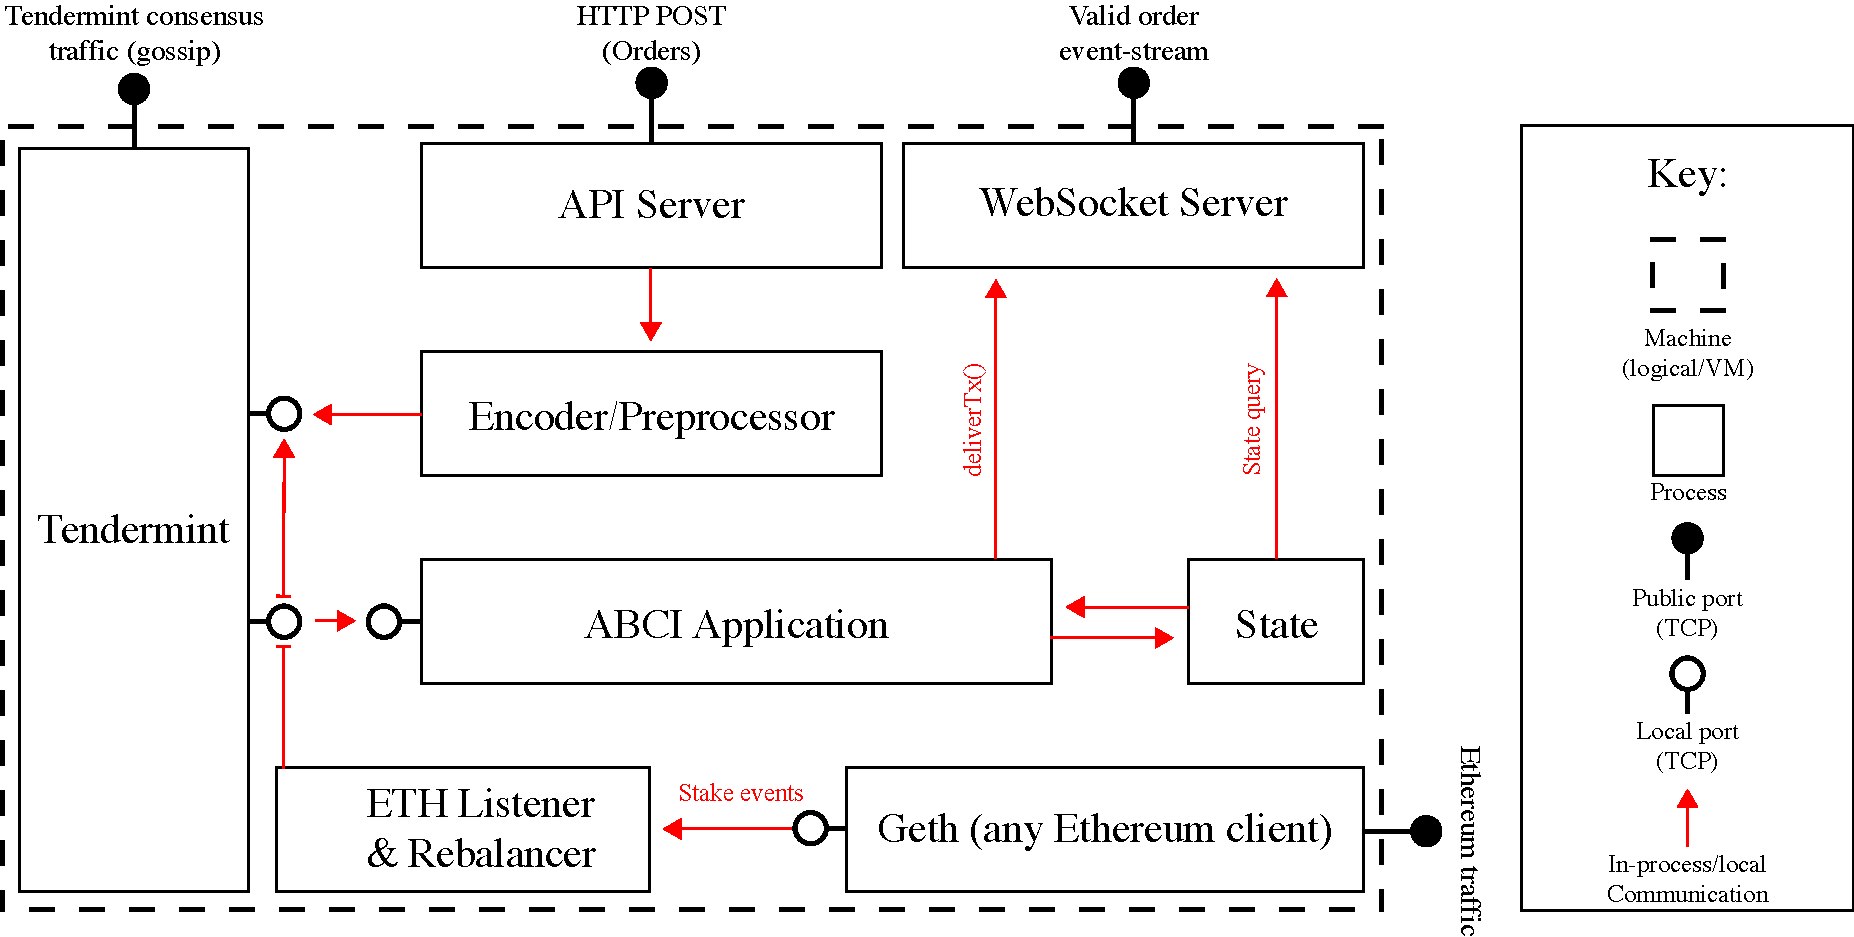
\includegraphics[scale=0.4]{../figures/fig3.pdf}
    \caption{Simplified process and port diagram of an OrderStream node, showing the required components. }
    \label{fig:fig3}
\end{figure}

\subsubsection{Network Architecture}\label{network architecture}

\noindent The OrderStream network itself is an organization of validator nodes running the ParadigmCore suite, initiated with the same Tendermint genesis\footnote{The Tendermint genesis.json files establishes the initial validator set of the network, but changes to the set can be made at the end of each consensus round.} file. The OrderStream network inherits the features of a Tendermint blockchain and network; it is Byzantine Fault Tolerant (BFT)\cite{bft} and has a high transactional throughput as the result of its PoS design and gossip protocol. A simplified diagram of the network’s organization into nodes and clusters is shown below (figure \ref{fig:fig4}). 

\begin{figure}[H]
    \centering
    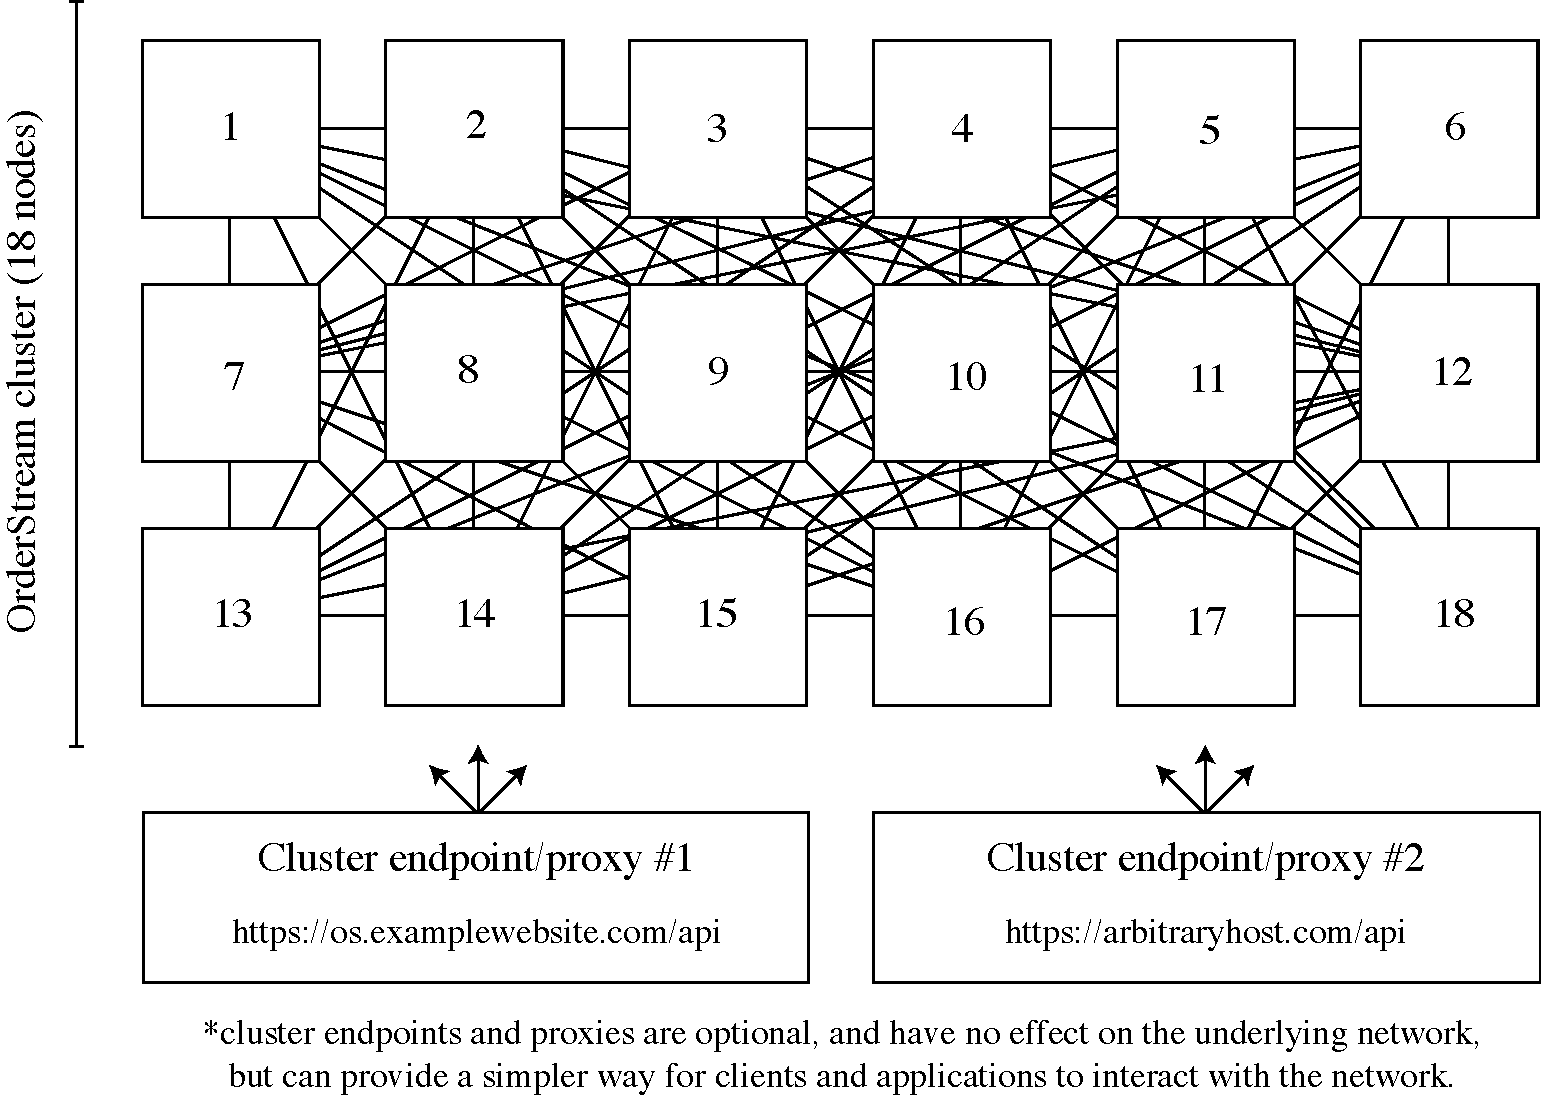
\includegraphics[scale=0.4]{../figures/fig4.pdf}
    \caption{Simplified network diagram of a 18 node OrderStream cluster, with 2 arbitrary public endpoints. }
    \label{fig:fig4}
\end{figure}

\subsection{State and Access Control}\label{staking}

\noindent In order to create sybil tolerance on Paradigm’s OrderStream network while preserving an incentive structure based purely on network topology (see section \ref{incentive model}), the network’s access control is based on a staking system. \\

\noindent The state of the machine/network is equivalent to the order limit mapping that is determined via the PosterStaking contract. The data structure maps an Ethereum address (key) to a stake size (value) which is then turned into a specific order limit by the OrderStream node software. Validator nodes act as witnesses and react to Ethereum events broadcast by the PosterStaking contract during a staking period and construct the mapping individually. At pre-defined time intervals (the end of a rebalancing period), an individual validator node will propose a new state for the network. 

\subsubsection{Formal Description}

\noindent During the staking period, nodes track and store stake/unstake events, and the associated staked amounts. To construct the new state and rate limit mapping, nodes compute the following function at the end of each rebalancing period for each address that has staked:

\begin{equation}
L_i = N_t * \frac{B_i}{B_T}
\end{equation}

\noindent Where $L_i$ is the rate limit for a given address, $N_t$ is the number of orders the network will accept\footnote{The total number of orders accepted during a given period must be computed based on the current network throughput, and can be increased or decreased via governance modules.} per period, $B_i$  is the staked balance for a given address $i$, and $B_T$ is the total staked balance in the contract. \\

\noindent After a predetermined confirmation threshold\footnote{A confirmation threshold is necessary to establish pseudo-finality for Ethereum events, as there is currently no concept of finality in Ethereum’s current PoW model.}, a validator submits the state proposal to other validators in a special ABCI transaction type. If other validators on the network agree on the new mapping ( the proposed mapping matches the one constructed locally), it is adopted by the network, and the updated mapping becomes the new state. \\

\noindent This process utilizes a shared security model as validator nodes are also event witnesses. It is also possible to design a slashing condition to enforce the validity of this process.

\subsection{Transaction Types}\label{transactions}
\noindent The actual commitment process for Tendermint, a RoundStep, requires the following sequence of states: NewHeight, Propose, Prevote, Precommit, and Commit\footnote{https://github.com/tendermint/tendermint/wiki/Byzantine-Consensus-Algorithm}. Each consensus round requires the same sequence of state changes. The OrderStream state machine will initially have three transactions types that can mutate the state. Below we identify these transaction types and categorize them by where the transaction proposal originates.

\subsubsection{Internal Transaction Type}

\noindent \underline{\texttt{RebalanceStake}}: this transaction type updates the state mapping based on events emitted from the PosterStaking contract, and can only be submitted by an active validator. One validator submits the proposal for the new state, and other validators vote to approve if it matches the mapping they have constructed locally for that rebalancing period.

\subsubsection{External Transaction Types}

\noindent \underline{\texttt{OrderBroadcast}}: this transaction type submits an order object for broadcast on the network. The validity of a particular transaction of this type is based on two factors, data structure and the network state, i.e. the poster has made the correct stake and has a non-zero order limit (\texttt{state.posterAddress.orderBroad\-castLimit > 0}). \\

\noindent \underline{\texttt{StreamBroadcast}}: this special transaction type defines a third party endpoint, specified by the poster, to which individuals can subscribe for an order feed without consensus induced latency. This relationship assumes some trust\footnote{Reputation systems can be built a layer above the OS network} to the poster. The validity of a transaction of StreamBroadcast type is based on the similar constraints as the OrderBroadcast transaction type. These constraints include data structure and StreamBroadcast transaction limit remaining (\texttt{state.posterAddress.streamBroadcastLimit > 0}). A poster that has made a stake is allowed one StreamBroadcast transaction per rebalancing period, regardless of stake size. Based on maker/taker dynamics within the market, we can assume the maker/poster will still submit OrderBroadcasts for individual orders to the main OS network. Makers (and posters acting as their agents) are economically incentivized to maximize the number of takers their order is discovered by. Thus, SubOrderStreams (third party order streams) exclusively provide advantage in edge cases.

\subsection{OrderBroadcast Transaction Data Model}\label{data model}
\subsubsection{Overview}
\noindent To ensure the OrderStream’s compatibility with orders for arbitrary settlement logic, it is necessary to create a simple yet adaptable data structure for network orders. The motivation for this model is to create an outer-level structure that OrderStream validator nodes can read and perform verification logic on, and an inner-level structure that contract developers can use to store any order data and signatures necessary for the execution of their settlement logic. 
 
\subsubsection{Data Structure Specification}
\noindent The high-level structure for orders is based around the JSON standard, but can be implemented as a generic map in any language that allows key-value pairs. This data structure is described below, with required and optional fields indicated. 

\begin{table}[h]
\centering
\caption{OrderStream OrderBroadcast transaction format }
\label{table:table1}
\begin{tabular}{|l|l|l|}
\hline
\textbf{Name} & \textbf{Data Type} & \textbf{Description} \\ \hline
\texttt{maker} & \texttt{string} & Optional - address of the order creator (or benefactor)\\ \hline
\texttt{subContract} & \texttt{string} & Required - contract address of target settlement logic \\ \hline
\texttt{makerArguments} & \texttt{[]object} & Optional - maker arguments specified by settlement logic  \\ \hline
\texttt{takerArguments} & \texttt{[]object} & Optional - taker arguments specified by settlement logic \\ \hline
\texttt{makerValues} & \texttt{object} & Required - maker order details (in key:value format) \\ \hline
\texttt{posterSignature} & \texttt{object} & Required - signature of the party that posted the order \\ \hline
\end{tabular}
\end{table}

\noindent The nested data structure outlined above provides flexibility that allows orders for arbitrary settlement logic to be relayed on the OrderStream network, all while ensuring validator nodes have access to the data they need to verify the order, without being concerned about the actual order details. The only field required for a validator node to approve or reject an order, is the \texttt{posterSignature}. Recovering the order poster's signature from the (\texttt{v, r, s, messageHex}) data in that field allows it to check the rate limit for that poster, which will exist and be nonzero if a stake was made. \\

\noindent Included in the appendix (section \ref{appendix}) is a fairly simple yet valid OrderStream order message. An order for more sophisticated settlement logic that does more than facilitate a simple swap of tokens will be more complicated.

\subsection{Network and Validator Incentive Model}\label{incentive model}

\subsubsection{Introduction}\label{incentive intro}

\noindent Traditional order books are nothing more than electronic lists of trade promises (buy/sell orders). Orders in Paradigm’s system, and hybrid decentralized systems more generally, are considerably more tangible. Instead of orders being represented by promises conforming to a centralized standard, they are cryptographically signed order messages executable by anyone. This characteristic is what directly enables Paradigm. Unlike centralized order books and trading venues, Paradigm is built on a decentralized network. The general protections of centralized systems provided by firewalls, infosec teams, and reputation-driven credentials are replaced with a BFT consensus protocol. \\

\noindent In any decentralized network, the economic and fault-tolerance models must be closely considered when designing the consensus protocol. The network must have a sufficient incentive structure to maintain market pressure on node hosts to behave properly, while at the same time maintaining fault-tolerance. Similarly, users must have an incentive to use the network over existing alternatives. With that said, it is unlikely significant market makers will ever opt for a decentralized feed trading venue over feeless centralized venues. \\

\noindent As a result, Paradigm’s OrderStream network’s consensus protocol must have an economic and fault-tolerance model that is specifically designed for a decentralized, performant, and fee-less environment.

\subsubsection{Tendermint and the OrderStream's Consensus Model}\label{consensus}

\noindent Paradigm uses the Tendermint protocol for consensus among OrderStream validator nodes. Tendermint is a Byzantine-fault tolerant state machine replication protocol that interfaces will applications like ParadigmCore via the Application Blockchain Interface (ABCI). Tendermint itself does not define an economic model. For Paradigm’s network there are two primary concerns with a fee-less architecture. First, sybil tolerance must be closely considered. For this, Paradigm introduces a staking system (more on the staking system and access control in section \ref{staking}). Second, the incentive model for validators must be considered. In order to incentivize validators to host the OrderStream network without introducing a fee structure, Paradigm introduces an incentive model based on the network’s topology. \\

\noindent As mentioned in the “matcher model” section (\ref{matcher model}), exchange systems and applications built on the OrderStream network require access to a validator node in order to write to the network. For many wishing to use the network, the easiest (or perhaps only) way to gain access to the network will be to host a validator node. Network participants may additionally create services (like Infura\footnote{https://infura.io/} for Ethereum) that provide API’s to allow remote and historical access to orders without hosting a node. \\

\noindent Applications facilitating a large volume through their interface, and thus through Paradigm’s network, will be incentivized to host an OrderStream validator based on the reduced read and write latency that results from using an on-site validator. 

\subsubsection{Formal Client and Validator Latency Models}\label{latency}
\noindent The latency for such systems is described more formally below. The network latency for a particular client, $i$, is defined as $N_i$, and the consensus latency of the network, which is constant, is defined as $C$. Total combined latency (including network and consensus) is indicated as $L_t$. The total collection of orders made via the OrderStream is defined as $M$, and a particular poster’s as $m_j$, where $m_j \subseteq M$. Consider the first case: latency for a client using the OrderStream:

\begin{equation}
M\ |\ L_t = n_i + c
\end{equation}

\noindent Conversely, we must also consider the latency for an OrderStream validator node, providing network access to some set of clients:

\begin{equation}
M\ |\ L_t = min(n_i) + c
\end{equation} 

\noindent Note the latency of a validator is always less than or equal to that of a client, which provides the primary incentive to host a node locally. We can also create latency models for subscription to the OrderStream and direct subscription to $m_j$ (for a client):

\begin{equation}
M - m_j\ |\ L_t = n_i + c 
\end{equation}
\begin{equation}
m_j\ |\ L_t = n_i
\end{equation}

\noindent As well as the related equation for an OrderStream validator node host's latency of a secondary stream:

\begin{equation}
M - m_j\ |\ L_t = min(n_i) + c 
\end{equation}
\begin{equation}
m_j\ |\ L_t = n_i
\end{equation}

\noindent Note that in this case, the potential minimum latency of a validator is always less than or equal to that of a client.

\subsubsection{A Note on Validator Nodes vs. Full Nodes}

\noindent Non-validator full nodes must utilize a validator node in a capacity similar to a client. In order to maintain incentives, validators should maintain closed\footnote{In reference implementations of the OrderStream network (such as ParadigmCore), mempool transaction gossip is disabled by default.} or privately networked mempools (disabling mempool transaction gossip) in order to maintain order privacy until after the transaction is included in a block. In this construction, a transaction will only be included in a block once the particular validator that accepted the transaction is selected as the round’s block producer. Thus, clients posting orders should direct transactions to as many validators as possible.

\subsection{Validator Integrity and Auditability}\label{integrity}
\noindent Paradigm will officially establish slashing conditions and bonding parameters for validators at a time closer to a complete network deployment. These conditions will ensure accountable safety and plausible liveness, resulting in the economic finality of transactions on the network. More generally, these conditions will discourage notable and explicit PoS network attacks. \\

\noindent While well designed slashing and finality conditions combine to provide strong network integrity, network participants must also consider attack vectors that are application specific, or less explicit in nature. In Paradigm’s system it is a client’s (or non-validating full node’s) responsibility to detect and react to such attacks. Generally these attacks will be a form of censorship, or advantage play by a validator or group of validators. A client should be able to design a clever and specific audit technique for the suspected malicious behavior. If a client is confident in their discovery, they can socialize their findings to the network in order to catalyze an update to the validator set.

\clearpage
\pagebreak
% END ORDERSTREAM SECTION


% BEGIN ORDERGATEWAY SECTION
\section{OrderGateway Forwarding Contract and Interface System}\label{contracts}

\subsection{Overview and Introduction}
\noindent Paradigm provides public access to a primary smart contract (the OrderGateway) deployed on the Ethereum network, which can be accessed directly via Ethereum’s web3.js API, or through application-layer software such as the JavaScript library being developed by Paradigm. The OrderGateway serves two primary functions. The first is to provide an interface platform for general contract logic (SubContracts) and wrappers (also SubContracts) implemented on the protocol. The second function the OrderGateway serves is to establish a high level canonical order/message schema that simplifies the process of concurrent multi-instrument trade execution for application developers. \\

\noindent An important distinction to make is that the use of the OrderGateway contract, and Paradigm’s contract system more generally, is not required to settle trades. Market takers can pull maker orders from the OrderStream network, and settle the trade directly through the SubContract. With that said, the OrderGateway is designed to make the processes and interactions involved in the settlement process more accessible. In the following sections, the components and functionality of Paradigm’s contract system will be explored in more detail.

\subsection{Protocol Contracts}
\noindent The PosterStaking contract (described more in section \ref{staking}) is the only Ethereum smart-contract that is completely essential to the relay protocol’s functionality. It serves as the guardian angel of the OrderStream network, preventing spam and making DDoS attacks to the network prohibitively expensive (sybil tolerance). The PosterStaking contract’s address must be known by all network validators, and should eventually be available for replacement and upgrade through decentralized governance modules (see section \ref{governance}). \\

\noindent All other protocol contracts essentially exist as convenience features, and can be used to simplify the trade process, or ignored in favor of custom systems. Regardless, Paradigm intends to release protocol contracts (such as an “official” OrderGateway contract) in addition to the PosterStaking contract concurrent with a full protocol launch.

\subsubsection{OrderGateway Contract}\label{ordergateway}
\noindent The OrderGateway is a simple smart-contract that allows arbitrary settlement logic to be executed through a single interface. A key value proposition of the Paradigm Protocol is that it enables support for the concurrent relay and settlement of arbitrarily sophisticated contract logic. \\

\noindent Since the relay protocol is agnostic to the underlying settlement logic being traded, additional complexity is offloaded to the market taker when the wish to fill a trade. Without a point of entry contract, market takers would be responsible for keeping track of various settlement logic interfaces. While this system would be usable, it is not ideal for developers who wish to build applications that support a wide variety of settlement logic. Developers would have to keep track of every allowed settlement contract, and provide interfaces for each of them. \\

\noindent The OrderGateway contract was introduced to alleviate the complexities of handling multiple contract interfaces side by side. The argument is that if a settlement contract conforms to a specific data interchange standard, takers can submit their trade to the OrderGateway (only needing the address of the target settlement logic) and it will be forwarded to the correct settlement contract. Another implication of this design is that it enables the creation of ‘wrapper’ contracts that allow the OrderGateway to interface with existing settlement logic – even contracts that predate Paradigm. SubContracts and settlement logic will be discussed in more detail in the next section. \\

\noindent A solidity implementation of the OrderGateway contract is included in section \ref{ordergateway code}, illustrating the contracts simplicity and forwarding functions. This example does not include features discussed in section \ref{ordergateway future}.

\subsection{SubContracts and Settlement Logic}
\subsubsection{Overview}
\noindent Without smart-contract based settlement logic, a protocol like Paradigm would not be useful. As such, settlement smart-contracts (called SubContracts in our system) are a key piece of the protocol, and are necessary for the system to have any utility. Although settlement contracts are necessary for protocol utility, in Paradigm’s system, they are entirely separated from the relay protocol itself. \\ 

\noindent The SubContract defines an interface to enforce function inclusion. This allows the OrderGateway to pass messages to any contract that implements the general SubContract interface. Orders relayed on the OrderStream network are defined for a specific SubContract, and the contract specified by the maker determines what the order format for both the maker and taker will look like. \\ 

\noindent Any type of smart-contract based settlement logic that implements a hybrid decentralized architecture (off-chain/arbitrary relay and on-chain settlement) can be relayed via Paradigm’s system. \\ 

\noindent Due to the design of the OrderGateway (described in section \ref{ordergateway}), not only can new contracts be created specifically for use with the Paradigm Protocol, but orders of existing contract-based settlement logic\footnote{Examples of existing hybrid decentralized exchange logic include 0x, dY/dX, Dharma, and b0x, among others.} can be traded through the protocol via the creation of “wrapping” SubContracts (described below).

\subsubsection{Native SubContracts}
\noindent A native SubContract is simply defined as settlement logic that has been specifically written for use with the Paradigm system, and the OrderGateway contract. Typically, this means the settlement pipeline for a native SubContract order will be two contracts; the trade will first pass through the OrderGateway, and is then executed by the native SubContract. \\

\noindent Native SubContracts accept a \texttt{bytes32} array for both the maker and taker arguments, which is unpacked inside the contract for settlement logic execution. A solidity implementation of the SubContract interface is included in section \ref{subcontract code}.

\subsubsection{Wrapping SubContracts}
\noindent In order to allow orders for existing settlement logic and contracts with non-standard interfaces to be settled through the OrderGateway contract, smart-contract “adapters” must be created. In Paradigm’s system, these contracts are called wrapping SubContracts. These wrapping contracts serve to convert the canonical input format established and expected by the OrderGateway, to whatever arbitrary input format is needed for the underlying settlement logic. \\

\noindent Wrapping SubContracts accept an input of two variable length \texttt{bytes32} arrays, as outputted from the OrderGateway. They are responsible for defining the internal logic necessary unpack the accepted byte arrays, perform additional parsing or verification, and then package the output to the format expected by the underlying contract the wrapper is written for. The OrderGateway simply passes along the maker and taker argument byte arrays from the initial \texttt{participate()} function call to the wrapper contract as if it were a native contract, where the wrapper contract then takes over. \\

\noindent Wrapping SubContracts allow orders for settlement logic with established and unchangeable data formats to be relayed and traded through Paradigm’s settlement pipeline without changes to their individual contracts. Wrapping SubContracts allow third-party and existing settlement logic to be traded through the OrderGateway alongside native SubContracts, providing greater simplicity for application developers wishing to support a wide variety of settlement logic side-by-side. \\

\noindent The settlement pipeline for a trade using a wrapping SubContract will be at least three contracts long, but can be longer depending on the contract and settlement pipeline the wrapper is written for.

\subsection{Filling Orders}
\noindent When a taker discovers a maker order they wish to fill from the OrderStream relay network, and decides to use Paradigm’s settlement process, they must set the correct allowances for the specific settlement SubContract specified by the maker in their order message. Once the correct allowances are set, the taker will submit the required taker order data (\texttt{takerValues}) and the \texttt{makerValues} to the \texttt{participate()} method of the OrderGateway contract. The order data includes the fields \texttt{methodId}, \texttt{data}, and \texttt{nonce} which are packaged into a byte array and submitted to the settlement logic on Ethereum via a signed transaction from the taker. \\

\noindent The Paradigm client libraries (called ParadigmConnect) provide classes and functions to simplify the process of taking of trades through the OrderGateway. We expect most application developers will use these libraries as drivers for the Paradigm Protocol to simplify trade execution, however there is no requirement to use Paradigm’s system to do so. Applications can build their own interfaces or submit taker orders for settlement manually if they wish. \\

\noindent Replay attack prevention is handled purely at the settlement layer (via hash mappings, incrementing counters, etc). The decision to exclude any replay attack prevention within the primary OrderGateway smart contract, is due to the fact that top-level mappings may be quasi-complete, as orders may be settled directly through a SubContract, never passing through the OrderGateway.

\clearpage
\pagebreak
% END ORDERGATEWAY SECTION


% BEGIN MATCHER MODEL SECTION
\section{The Matcher Model}\label{matcher model}
\noindent With the creation of a relay protocol, the existing “relayer” model for hybrid decentralized settlement logic must be reconsidered. The role of a relayer in Paradigm’s model becomes further abstracted to the protocol and infrastructure layers. External and independent systems are no longer fundamentally responsible for order broadcast and discovery. Instead, external systems become solely responsible for trade execution. \\
 
\noindent Consuming entities (exchange systems/services) will subscribe to the OrderStream and derive a subset (database) of orders. Exchange systems can then use this subset of orders to accurately suggest maker orders to a network of urgent market participants, specifically takers. Matchers distinguish themselves primarily based on trade execution practices. Competition between matchers will likely be driven by distinguishing parameters such as order price, matching speed, execution speed, user experience and API strength. Sophisticated matchers should perform their own secondary order book maintenance to reduce the number of order collisions during the settlement process and, in turn, provide the most accurate and stable matching service. Matchers may also choose to tailor their service to specific instrument or asset offerings. \\ 

\noindent In general, the matcher model aims to replace proprietary liquidity with global liquidity, encouraging borderless and efficient global markets with low barriers to entry for all market agents.

\clearpage
\pagebreak
% END MATCHER MODEL SECTION


% BEGIN GOVERNANCE SECTION
\section{Protocol Governance and Decentralization}\label{governance}
\noindent Many of the processes and systems described in this paper require some form of decentralized governance. These processes include network access control, contract upgrades, validator election/removal, and general protocol governance. Most of these processes will not be fully implemented until later versions of the protocol are released, but the design of these systems remains an area of active research. We are also exploring the possibility of a native token for our protocol. \\ 

\noindent We plan to work closely with experts in relevant fields, and involve the community in any decisions concerning a token, token mechanics, token distribution, etc. For now, our focus remains on developing and deploying a functional system that may or may not motivate the creation of a native token for protocol governance, core systems, and incentive structure.

\clearpage
\pagebreak
% END GOVERNANCE SECTION


% BEGIN FUTURE WORK 
\section{Future Work}\label{future work}
\subsection{Decentralized Trade Execution}
\noindent In addition to order broadcast and discovery, we imagine the OrderStream network and contract implementations can be expanded to include trade execution functionality; particularly the ability to effectively cancel orders off-chain. The proposed system would essentially function as a decentralized trade execution coordinator, establishing an ordering for special transaction types on the OrderStream network. This ordering could be enforced on-chain during a settlement period via agent submitted cryptographic proofs. \\

\noindent The implementation of this system would be optional. In Paradigm’s current architecture, message relay is intentionally separated from order settlement. The OrderStream network was not designed to handle assets; the network makes specific tradeoffs in order to optimize the process of order relay, not trade settlement. The implementation of cancel functionality opens additional attack vectors from potentially malicious validators. Such functionality should be approached with the understanding that execution coordination assumes considerably more trust than order relay.

\subsection{OrderGateway Upgrades and Expansion}\label{ordergateway future}
\noindent The OrderGateway contract also offers avenues for future upgrades and feature addition. One potential upgrade would be the ability to distribute fees to SubContracts based on a specified fee schedule. This application would be primarily for native SubContracts as they could most easily require orders to pass through the OrderGateway contract during settlement. Unfortunately, due to the public nature of Ethereum, the defensibility of fee structures within smart contracts is limited. With that said, some decrementing fee structure might be feasible. \\

\noindent The OrderGateway could also be used to emit events that help with order book maintenance. Such a system would involve tracking complete or partial fills of certain SubContracts, and emitting events that can be picked up by applications and services to update their order books. This system would work most effectively with native SubContracts, but would be possible with wrapper contracts as well.

\clearpage
\pagebreak
% END FUTURE WORK


% BEGIN ACKNOWLEDGEMENTS SECTION
\section{Acknowledgements}\label{acknowledgements}
\noindent We would like to thank Nick Freyaldenhoven and Stephen Fiser for their feedback and revisions to this paper, and their continued work on the Paradigm Project and smart contract system. Without their early and continued work on the protocol, Paradigm would not be possible. \\ 

\noindent We also want to express our gratitude for those in the Ethereum and decentralized finance communities who have worked to create technologies and developer tooling for web3 infrastructure. The utility of a system like Paradigm is largely dependant upon the work of teams building settlement primitives that collectively enable a decentralized financial system.

\clearpage
\pagebreak
% END ACKNOWLEDGEMENTS SECTION


% BEGIN APPENDIX SECTION
\section{Appendix}\label{appendix}

\subsection{Paradigm-specific Terminology}
\begin{enumerate}
\item \underline{OrderStream}: a decentralized, event-based relay network for orders of hybrid-decentralized settlement logic. 
\item \underline{OrderGateway}: a forwarding smart-contract interface that simplifies the process of settling trades. 
\item \underline{SubContract}: a general term for settlement logic smart-contracts in the Paradigm system.
\item \underline{PosterStaking Contract}: a smart-contract that market posters (or makers) must deposit a stake to in order to gain access to the OrderStream network.
\item \underline{OrderStream Node}: a logical or virtual machine running the OrderStream network node software (ParadigmCore).
\item \underline{OrderStream Validator}: an OrderStream node that has a public/private key included in the current validator set. Proposes and votes on blocks. 
\item \underline{Maker}: a market agent creating unfilled orders for the OrderStream network.
\item \underline{Taker}: a market agent filling maker orders from the OrderStream network.
\item \underline{Poster}: the party that has made a stake in the PosterStaking contract. Responsible for posting maker orders, and can be the same as the maker.
\end{enumerate}

\subsection{Third-party Software and Protocols}
\begin{enumerate}
\item \underline{Tendermint}: a byzantine fault tolerant state machine replication software.
\item \underline{0x}: a protocol that facilitates smart-contract based decentralized exchange.
\item \underline{Dharma}: a decentralized lending and debt protocol.
\item \underline{dY/dX}: a decentralized margin trading and derivatives protocol.
\item \underline{b0x}: a decentralized lending and margin trading protocol.
\end{enumerate}

\subsection{Code and Order Examples}
\noindent Included in this section examples of Solidity implementations of the OrderGateway and SubContract interfaces, as well as a JSON example of a valid order as relayed on the OrderStream network. The OrderGateway and SubContract examples represent the current implementations of those contracts at the time of this paper's publication, however both are still in development and will likely undergo further revision as the protocol matures and features are added.

\subsubsection{OrderGateway Specification (Solidity)}\label{ordergateway code}
\begin{lstlisting}[language=Solidity]
pragma solidity ^0.4.24;

import "paradigm-solidity/contracts/SubContract.sol";

contract OrderGateway {

    constructor() public {}

    function participate(address subContract, bytes32[] makerData, bytes32[] takerData) public returns (bool) {
        return SubContract(subContract).participate(makerData, takerData);
    }

    function makerArguments(address subContract) public view returns (string) {
        return SubContract(subContract).makerArguments();
    }

    function takerArguments(address subContract) public view returns (string) {
        return SubContract(subContract).takerArguments();
    }
}
\end{lstlisting}

\subsubsection{SubContract Interface Specification (Solidity)}\label{subcontract code}
\begin{lstlisting}[language=Solidity]
pragma solidity ^0.4.24;

import "openzeppelin-solidity/contracts/math/SafeMath.sol";

contract SubContract {
    using SafeMath for uint;

    string public makerArguments;
    string public takerArguments;

    function participate(bytes32[] makerData, bytes32[] takerData) public returns (bool);

    function ratioFor(uint value, uint numerator, uint denominator) internal pure returns (uint) {
        return value.mul(numerator).div(denominator);
    }
}
\end{lstlisting}

\subsubsection{OrderStream Data Model Example (JSON)}
\begin{lstlisting}
{
   "maker": "0x300bd2d65d490d1adc4218247a215e3efcfdbd88",
   "subContract": "0xP8c77482e45F2F44dC1745X52C74426C631bdD52",
   "makerArguments": [{ "name": "maker", "dataType": "address" }],
   "takerArguments": [{ "name": "taker", "dataType": "address" }],
   "makerValues": {
      "maker": "0x400bd2d65d490d1ebc3518247a215e3efcfdbd79",
      "sigV": 27,
      "sigR": "0xa3b2b902d1ff66595b59452459dc5548de6d32d3bdce1a680d23",
      "sigS": "0x3a905abbad1efea2ae02f19cb5e115414b07fc95868d84a634d0"
   },
   "posterSignature": {
      "v": 27,
      "r": "0xa3b2b902d1ff66595b59452459dc5548de6d32d3bdce1a680d23",
      "s": "0x3a905abbad1efea2ae02f19cb5e115414b07fc95868d84a634d0"
   }
}
\end{lstlisting} 

\clearpage
\pagebreak
% END APPENDIX SECTION

% BEGIN BIBLIOGRAPHY
\begin{thebibliography}{9}

\bibitem{defi}
Max Bronstein. "Mapping the Decentralized Financial System,"
\\\texttt{https://tokeneconomy.co/mapping-the-decentralized-financial-system-7c5af65e0335}

\bibitem{0xwhitepaper}
Will Warren, Amir Bandeali. "0x: An Open Protocol for Decentralized Exchange on the Ethereum Blockchain,"
\\\texttt{https://0xproject.com/pdfs/0x\_white\_paper.pdf}

\bibitem{dydxwhitepaper}
Antonio Juliano. "dYdX: A Standard for Decentralized Margin Trading and Derivatives,"
\\\texttt{https://whitepaper.dydx.exchange/}

\bibitem{dharmawhitepaper}
Nadav Hollander. "Dharma: A Generic Protocol for Tokenized Debt Issuance,"
\\\texttt{https://whitepaper.dharma.io/}

\bibitem{globalliquidity}
Liam Kovatch. "Global Liquidity, Motivated,"
\\\texttt{https://medium.com/paradigm-foundation/global-liquidity-motivated-b334c2ea19e1}

\bibitem{eufinance}
Official Journal of the European Union. "On Markets in Financial Instruments,"
\\\texttt{https://eur-lex.europa.eu/legal\-content/EN/TXT/PDF/?uri$=$CELEX$:$32014R0600\&from$=$EN}
\\ Article (2)(1)(45)

\bibitem{relayerideas}
Tom Schmidt. "18 Ideas for 0x Relayers in 2018,"
\\\texttt{https://blog.0xproject.com/18-ideas-for-0x-relayers-in-2018-80a1498b955f}

\bibitem{tendermint}
Tendermint. "Tendermint Wiki,"
\\\texttt{https://github.com/tendermint/tendermint/wiki}

\bibitem{abcispec}
Tendermint. "Tendermint Application Blockchain Interface Specification,"
\\\texttt{https://tendermint.com/docs/spec/abci/abci.html}

\bibitem{bft}
Leslie Lamport, Robert Shostak, Marshall Pease. "The Byzantine Generals Problem,"
\textit{ACM Transactions on Programming Languages and Systems, }Vol. 4, No. 3. July 1982. Pages 382-401.


\end{thebibliography}
% END BIBLIOGRAPHY

\end{document}